% SC2008 --- Chapter 6: Link Layer -- Ethernet, MAC, ARP, Switches (0->100)
\chapter{Link Layer: Ethernet, MAC, ARP and Switching}\label{ch:link}
\begin{quote}
\emph{``The link delivers frames to neighbours; the network delivers packets to the world.''} --- Every IP packet rides inside a link-layer frame for one hop at a time.
\end{quote}
\noindent\fbox{\parbox{\dimexpr\linewidth-2\fboxsep-2\fboxrule}{%
\textbf{From zero: we build here, no prior framing assumed.} We start from ``how do two machines share a wire?'' with pictures before headers. Every notion---frame, MAC address, ARP, CSMA/CD, switch table, VLAN---is defined on first use and linked to the IP layer above. No link-layer background is assumed.}}
\vspace{0.4em}
\section*{Learning Outcomes}
After this chapter you will be able to:
\begin{enumerate}[label=(L\arabic*)]
    \item explain link-layer services: framing, error detection, and reliable delivery;
    \item distinguish MAC from IP addresses and describe ARP resolution and caching;
    \item describe Ethernet framing, addressing, and CSMA/CD with exponential backoff;
    \item explain how switches self-learn, forward, filter, and support VLANs;
    \item contrast hubs, switches, and routers in terms of collision vs.\ broadcast domains.
\end{enumerate}
% ============================================================
\section{What the Link Layer Does}\label{sec:link-services}
The network layer hands a datagram to the link layer, which must move it \emph{one hop} to the next node. Think of a courier van between two adjacent post offices: it wraps the envelope (IP packet) in a van manifest (frame header/trailer), drives it one segment, unwraps at the next office.
\emph{Services:} framing (delimit where frame starts/ends), error detection (CRC), optional reliable delivery (rare on wired links---left to TCP), flow control, and medium access (who talks when). Framing is non-trivial: the receiver must find frame boundaries in a continuous bit stream. Ethernet uses preamble + length/Type; HDLC uses bit stuffing with flags \texttt{01111110}.
\begin{figure}[h]
\centering
\resizebox{\linewidth}{!}{%
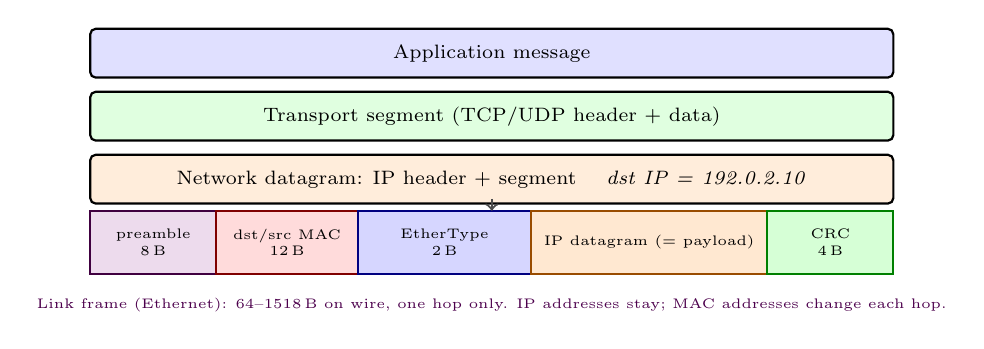
\begin{tikzpicture}[every node/.style={font=\scriptsize},
  layer/.style={draw, thick, rounded corners=2pt, minimum height=0.62cm, align=center}]
\node[layer, fill=blue!12, minimum width=10.2cm] (app) at (5.1,1.85) {Application message};
\node[layer, fill=green!12, minimum width=10.2cm] (trans) at (5.1,1.05) {Transport segment (TCP/UDP header + data)};
\node[layer, fill=orange!14, minimum width=10.2cm] (net) at (5.1,0.25) {Network datagram: IP header + segment \quad \emph{dst IP = 192.0.2.10}};
\draw[fill=violet!14, draw=violet!50!black, thick] (0,-0.95) rectangle (1.6,-0.15);
\node[font=\tiny, align=center] at (0.8,-0.55) {preamble\\{\tiny 8\,B}};
\draw[fill=red!14, draw=red!50!black, thick] (1.6,-0.95) rectangle (3.4,-0.15);
\node[font=\tiny, align=center] at (2.5,-0.55) {dst/src MAC\\{\tiny 12\,B}};
\draw[fill=blue!16, draw=blue!50!black, thick] (3.4,-0.95) rectangle (5.6,-0.15);
\node[font=\tiny, align=center] at (4.5,-0.55) {EtherType\\{\tiny 2\,B}};
\draw[fill=orange!18, draw=orange!60!black, thick] (5.6,-0.95) rectangle (8.6,-0.15);
\node[font=\tiny, align=center] at (7.1,-0.55) {IP datagram (= payload)};
\draw[fill=green!16, draw=green!50!black, thick] (8.6,-0.95) rectangle (10.2,-0.15);
\node[font=\tiny, align=center] at (9.4,-0.55) {CRC\\{\tiny 4\,B}};
\node[font=\tiny, violet!60!black] at (5.1,-1.35) {Link frame (Ethernet): 64--1518\,B on wire, one hop only. IP addresses stay; MAC addresses change each hop.};
\draw[->, thick, gray!60!black] (5.1,0.0) -- (5.1,-0.15);
\end{tikzpicture}}%
\caption{Encapsulation: IP datagram becomes the payload of an Ethernet frame. Each hop re-wraps with new MAC addresses.}
\label{fig:link-encapsulation}
\end{figure}
Key idea: \emph{IP addresses are end-to-end (unchanged); MAC addresses are hop-by-hop (rewritten by each router)}. A router strips the incoming frame's MAC header, looks up the IP, and builds a new frame with its own MAC as source and next-hop's MAC as destination. Encapsulation overhead matters: Ethernet adds 18\,B header/trailer + 8\,B preamble, so a 1500\,B IP packet becomes 1526\,B on wire (plus inter-frame gap 12\,B).
Error detection: parity catches odd bit flips; Internet checksum catches many bursts; \emph{CRC-32} (Ethernet) divides the bit stream by a generator polynomial and appends the remainder---detects all bursts $<32$ bits and any odd number of errors. Bad CRC $\to$ drop; no retransmission at link layer on wired links (wireless 802.11 does retransmit).
\section{MAC Addresses and ARP}\label{sec:mac-arp}
A \emph{MAC address} (Media Access Control) is a 48-bit identifier burned into each network interface (NIC), written as hex: \texttt{1A:2B:3C:4D:5E:6F}. Uniqueness via OUI (first 24 bits = vendor). Broadcast address is \texttt{FF:FF:FF:FF:FF:FF}. Unlike IP, MAC is flat---no hierarchy, no aggregation, hence not routable beyond one LAN.
IP and MAC solve different problems: IP is hierarchical and routable (like postal code); MAC is flat and local (like serial number on the van). To send an IP datagram on a link, the sender must know the \emph{next-hop MAC}.
\emph{ARP} (Address Resolution Protocol) maps IP $\to$ MAC within a subnet. Hosts also use DHCP to \emph{obtain} their own IP; ARP then resolves neighbours.
\begin{figure}[h]
\centering
\resizebox{0.96\linewidth}{!}{%
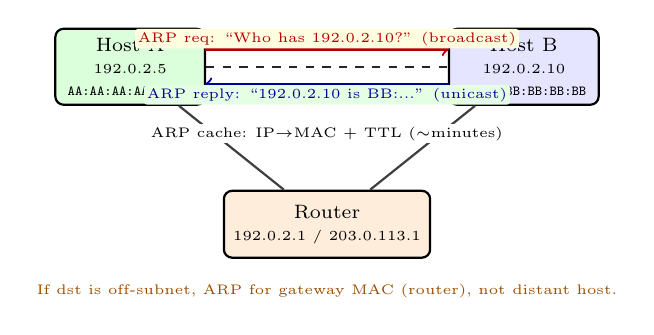
\begin{tikzpicture}[every node/.style={font=\scriptsize},
  host/.style={draw, thick, rounded corners=3pt, fill=blue!10, minimum width=1.9cm, minimum height=0.85cm, align=center},
  rtr/.style={draw, thick, rounded corners=3pt, fill=orange!14, minimum width=1.7cm, minimum height=0.85cm, align=center}]
\node[host, fill=green!14] (A) at (0,0) {Host A\\{\tiny 192.0.2.5}\\{\tiny \texttt{AA:AA:AA:AA:AA:AA}}};
\node[host] (B) at (5.0,0) {Host B\\{\tiny 192.0.2.10}\\{\tiny \texttt{BB:BB:BB:BB:BB:BB}}};
\node[rtr] (R) at (2.5,-2.0) {Router\\{\tiny 192.0.2.1 / 203.0.113.1}};
\draw[thick, gray!50!black] (A) -- (R) -- (B);
\draw[thick, gray!30!black, dashed] (A) -- (B);
\draw[->, thick, red!70!black] (0.95,0.22) -- (4.05,0.22) node[midway, above, font=\tiny, fill=yellow!12, rounded corners=1pt, inner sep=1pt] {ARP req: ``Who has 192.0.2.10?'' (broadcast)};
\draw[->, thick, blue!60!black] (4.05,-0.22) -- (0.95,-0.22) node[midway, below, font=\tiny, fill=green!10, rounded corners=1pt, inner sep=1pt] {ARP reply: ``192.0.2.10 is BB:...'' (unicast)};
\node[font=\tiny, fill=white, inner sep=1pt] at (2.5,-0.85) {ARP cache: IP$\to$MAC + TTL ($\sim$minutes)};
\node[font=\tiny, orange!60!black] at (2.5,-2.85) {If dst is off-subnet, ARP for gateway MAC (router), not distant host.};
\end{tikzpicture}}%
\caption{ARP in a subnet: A broadcasts a request; B unicasts a reply. Both cache the mapping to avoid future broadcasts.}
\label{fig:arp}
\end{figure}
\begin{definition}[ARP cache]\label{def:arp-cache}
Each host/router maintains a table $\text{IP}\mapsto(\text{MAC},\text{TTL})$. On miss, it broadcasts an ARP request; the owner replies. Entries expire (typically 2--20\,min) to handle NIC changes. Gratuitous ARP (announce own mapping) detects duplicate IPs.
\end{definition}
\begin{lstlisting}[language=Python]
# Simplified ARP cache with TTL
import time
arp_cache = {}  # ip_str -> (mac_str, expiry)
TTL = 300  # seconds
def arp_lookup(ip):
    entry = arp_cache.get(ip)
    if entry and entry[1] > time.time():
        return entry[0]
    return None  # -> broadcast ARP request

def arp_update(ip, mac):
    arp_cache[ip] = (mac, time.time() + TTL)

def send_datagram(dst_ip, payload):
    mac = arp_lookup(dst_ip)
    if mac is None:
        print(f"ARP broadcast: who has {dst_ip}?")
        # ... wait for reply, then arp_update(dst_ip, reply_mac)
    # build Ethernet frame with dst MAC and send
\end{lstlisting}
If destination is outside the subnet, the sender ARPs for the \emph{gateway} (first-hop router) MAC and sends the frame there; the router forwards via IP. This is why ``default gateway'' is configured---it is the next-hop MAC for all off-subnet traffic. ARP spoofing (forged replies) enables MITM; static entries and Dynamic ARP Inspection mitigate it.
\section{Ethernet and CSMA/CD}\label{sec:ethernet}
Ethernet (IEEE 802.3) is the dominant wired link. Frame format (excluding preamble): dst\,MAC (6\,B) $\vert$ src\,MAC (6\,B) $\vert$ EtherType (2\,B) $\vert$ payload (46--1500\,B) $\vert$ CRC (4\,B). Payload $<$46\,B is padded to meet 64\,B minimum (collision detection needs a minimum frame time of 64\,B $\times$ 8 / rate). EtherType says what is inside: \texttt{0x0800}=IPv4, \texttt{0x86DD}=IPv6, \texttt{0x0806}=ARP.
Medium access: classic Ethernet is a \emph{broadcast medium} (coax, or hub). Who may transmit? \emph{CSMA/CD} (Carrier Sense Multiple Access with Collision Detection):
\begin{enumerate}[label=(\alph*), itemsep=0.3em]
    \item Carrier sense: listen; if idle, transmit; if busy, wait.
    \item Collision detection: while transmitting, listen; if collision (voltage spike), abort and jam.
    \item Exponential backoff: after $k$th collision, pick random $r\in\{0,\dots,2^{k}-1\}$ (capped at $k=10$), wait $r\times512$ bit-times, retry ($k\le16$ else drop).
\end{enumerate}
\begin{center}
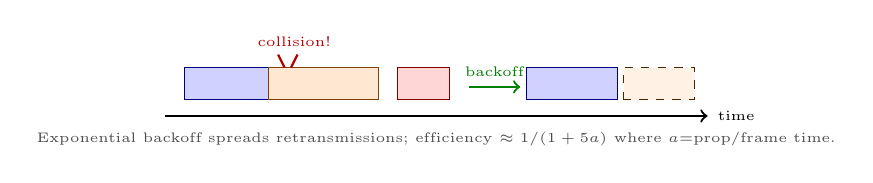
\begin{tikzpicture}[scale=0.82, every node/.style={font=\scriptsize}]
\draw[->, thick] (0,0) -- (8.4,0) node[right, font=\tiny] {time};
\fill[blue!18, draw=blue!50!black] (0.3,0.25) rectangle (2.0,0.75) node[midway, font=\tiny] {A sends};
\fill[orange!18, draw=orange!50!black] (1.6,0.25) rectangle (3.3,0.75) node[midway, font=\tiny] {B sends};
\node[font=\tiny, red!70!black] at (2.0,1.15) {collision!};
\draw[thick, red!70!black] (1.85,0.75) -- (1.75,0.95);
\draw[thick, red!70!black] (1.95,0.75) -- (2.05,0.95);
\fill[red!16, draw=red!50!black] (3.6,0.25) rectangle (4.4,0.75) node[midway, font=\tiny] {jam};
\draw[->, thick, green!50!black] (4.7,0.45) -- (5.5,0.45) node[midway, above, font=\tiny] {backoff};
\fill[blue!18, draw=blue!50!black] (5.6,0.25) rectangle (7.0,0.75) node[midway, font=\tiny] {A retry};
\fill[orange!10, draw=orange!30!black, dashed] (7.1,0.25) rectangle (8.2,0.75) node[midway, font=\tiny] {B waits};
\node[font=\tiny, gray!60!black] at (4.2,-0.35) {Exponential backoff spreads retransmissions; efficiency $\approx 1/(1+5a)$ where $a$=prop/frame time.};
\end{tikzpicture}
\end{center}
Modern switched Ethernet is full-duplex with no collisions---CSMA/CD remains only as a fallback and for Wi-Fi's cousin CSMA/CA (which avoids rather than detects collisions). Efficiency intuition: $a$= propagation / transmission time; if $a$ is small, channel is idle quickly and efficiency is high. Switched links with $a\to0$ approach 100\% utilisation.
CRC-32 detects bit errors; bad frames are dropped (no retransmission at link layer---TCP will handle it). A 10\,Gbps link with BER $10^{-12}$ still sees a bad frame every few seconds at full rate, so CRC is essential.
\section{Switches, Learning, and VLANs}\label{sec:switches}
A \emph{hub} repeats bits to all ports (one collision domain). A \emph{switch} is smarter: it has a \emph{forwarding table} mapping MAC $\to$ port, built by \emph{self-learning}. Unlike a router (IP table via routing protocols), a switch needs no configuration.
\emph{Learning:} when a frame arrives on port $p$ with source MAC $s$, record $(s\to p)$. \emph{Forwarding:} look up destination MAC $d$: if found and $p'\neq p$, forward only to $p'$ (filtering); if unknown, flood to all ports except $p$; if $p'=p$, drop (same segment). Entries age out ($\sim$5\,min). No configuration needed---plug and play.
\begin{figure}[h]
\centering
\resizebox{\linewidth}{!}{%
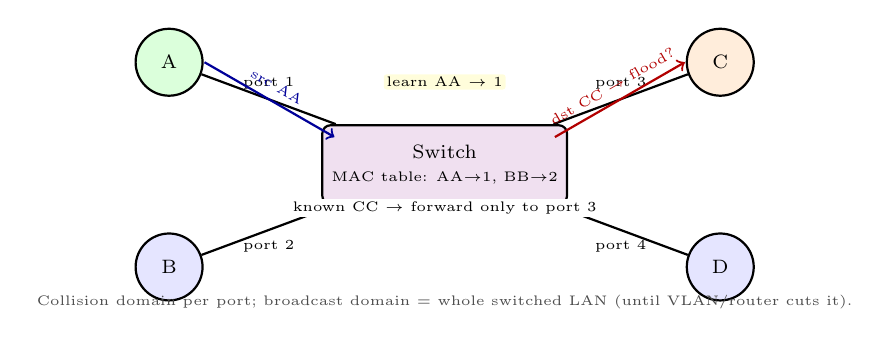
\begin{tikzpicture}[every node/.style={font=\scriptsize},
  sw/.style={draw, thick, fill=violet!12, minimum width=2.8cm, minimum height=1.0cm, align=center, rounded corners=3pt},
  host/.style={draw, thick, circle, fill=blue!10, minimum size=0.85cm, inner sep=1pt}]
\node[sw] (S) at (3.5,0) {Switch\\{\tiny MAC table: AA$\to$1, BB$\to$2}};
\node[host, fill=green!14] (A) at (0,1.3) {A};
\node[host] (B) at (0,-1.3) {B};
\node[host, fill=orange!14] (C) at (7,1.3) {C};
\node[host] (D) at (7,-1.3) {D};
\draw[thick] (A) -- node[above, font=\tiny] {port 1} (S);
\draw[thick] (B) -- node[below, font=\tiny] {port 2} (S);
\draw[thick] (S) -- node[above, font=\tiny] {port 3} (C);
\draw[thick] (S) -- node[below, font=\tiny] {port 4} (D);
\draw[->, thick, blue!60!black] (0.45,1.3) -- (2.1,0.35) node[midway, sloped, above, font=\tiny] {src AA};
\node[font=\tiny, fill=yellow!14, rounded corners=1pt, inner sep=1pt] at (3.5,1.05) {learn AA $\to$ 1};
\draw[->, thick, red!70!black] (4.9,0.35) -- (6.55,1.3) node[midway, sloped, above, font=\tiny] {dst CC $\to$ flood?};
\node[font=\tiny, fill=white, inner sep=1pt] at (3.5,-0.55) {known CC $\to$ forward only to port 3};
\node[font=\tiny, gray!60!black] at (3.5,-1.75) {Collision domain per port; broadcast domain = whole switched LAN (until VLAN/router cuts it).};
\end{tikzpicture}}%
\caption{Self-learning switch: learns source MACs, forwards by destination lookup. Unknown destinations are flooded; learning makes future frames unicast.}
\label{fig:switch-learning}
\end{figure}
\begin{lstlisting}[language=Python]
class Switch:
    def __init__(self, n_ports): self.table={}; self.n=n_ports
    def receive(self, frame, in_port):
        self.table[frame.src] = in_port          # learn source
        out = self.table.get(frame.dst)
        if out is None:          # unknown -> flood
            return [p for p in range(self.n) if p!=in_port]
        elif out == in_port:     # same segment -> filter
            return []
        else:                    # known -> unicast forward
            return [out]

# Example: A->B then B->A
sw = Switch(4)
print(sw.receive(type('F',(),{'src':'AA','dst':'BB'})(),0))  # flood [1,2,3]
print(sw.table)  # {'AA':0}
print(sw.receive(type('F',(),{'src':'BB','dst':'AA'})(),1))  # [0]
\end{lstlisting}
Switches create \emph{per-port collision domains} but still one \emph{broadcast domain}. To isolate broadcast, use \emph{VLANs} (IEEE 802.1Q): tag frames with 12-bit VLAN ID (4\,B extra header between src MAC and EtherType), switch forwards only within the same VLAN---as if multiple virtual switches. A trunk port carries multiple VLANs tagged; an access port belongs to one VLAN untagged. Routers (or L3 switches) connect VLANs at layer 3.
\emph{Hub vs.\ switch vs.\ router:} hub = physical layer (repeats, one collision, one broadcast); switch = link layer (learns, many collisions isolated, one broadcast/VLAN); router = network layer (routes by IP, cuts both collision and broadcast domains). Loops between switches need Spanning Tree Protocol (STP) to prune to a tree; otherwise flooded frames loop forever.
\section{Putting It Together: A Frame's Life One Hop}\label{sec:frame-life}
Follow a datagram from router R1 to host B across Ethernet. R1 has IP datagram for \texttt{192.0.2.10} and knows next-hop is directly connected on \texttt{eth0} (\texttt{192.0.2.1/24}).
It checks ARP cache for \texttt{192.0.2.10}: miss, so it broadcasts \texttt{Who has 192.0.2.10?}
B replies with its MAC; both cache the binding.
R1 now builds the frame: dst MAC = B, src MAC = R1-eth0, EtherType = \texttt{0x0800}, payload = IP datagram, CRC appended.
It transmits: on switched full-duplex, no CSMA/CD contention; on a hub, it would sense and back off.
Switch S2 receives on port 2, learns \texttt{R1-MAC $\to$ 2}, looks up \texttt{B-MAC}: if known on port 4, forwards only there; if unknown, floods.
B's NIC checks dst MAC matches (or broadcast), verifies CRC, strips header, hands IP datagram to Network layer.
On the reverse path, B will already have R1's MAC cached, so no ARP is needed---one broadcast serves many packets until TTL expiry.

Aggregation examples: two /24s aggregate to a /23 (512 addresses), two /23s to a /22 (1024), and ISP block 	exttt{14.24.0.0/15} holds 131\,072. This hierarchy keeps the global BGP table tractable.

\begin{remark}[Why no IP routing on a switch?]
A switch never looks at the IP address; it forwards by MAC table built from observing sources.
This makes it plug-and-play but also broadcast-heavy. A router, by contrast, forwards by IP prefix and cuts broadcasts.
That is why large LANs are segmented into VLANs (L2 isolation) connected by routers (L3).
\end{remark}

Error case: CRC fails (bit error on wire). The switch or host drops the frame silently. No link-layer retransmission on wired Ethernet---IP also does not retransmit. TCP at the endpoints will timeout and retransmit, illustrating layering: reliability only where it is end-to-end.


A quick lab check: run \texttt{arp -a} to see cached bindings, \texttt{ip link} to see MACs, and capture with Wireshark to inspect Ethernet II headers and the EtherType field. Compare the MAC addresses hop-by-hop with the unchanged IP addresses.

Spanning Tree note: with redundant switches, STP elects a root, blocks one port to break the loop, and unblocks on failure. Without STP, a single broadcast frame would loop forever and multiply exponentially (broadcast storm).

\section{Chapter Notes}
Ethernet v2 / IEEE 802.3, ARP in RFC\,826, VLANs in 802.1Q, STP in 802.1D. Kurose--Ross Ch.~6 and Peterson--Davie cover Ethernet evolution from 10\,Mbps coax to 400\,Gbps switched full-duplex. Wireshark captures make headers concrete---try \texttt{arp -a} and inspect \texttt{Ethernet II} headers in any capture.
\section{Exercises}\label{sec:ch06-exercises}
\begin{enumerate}[label=E6.\arabic*, leftmargin=*, itemsep=0.7em]
    \item \textbf{MAC vs.\ IP.} Host A (IP$_A$, MAC$_A$) sends to B (IP$_B$, MAC$_B$) via router R (MAC$_R$ left, MAC$_R'$ right). List src/dst IP and MAC at each hop for A$\to$R$\to$B. Which addresses change and which do not? Why must MAC change?
    \item \textbf{ARP cache.} A pings B for the first time in a /24. Describe each ARP message, who broadcasts, who replies, and what each cache contains after. What happens on the second ping? When would an entry expire or be overwritten?
    \item \textbf{Ethernet overhead.} A 40\,B TCP ACK (20\,B IP + 20\,B TCP) is sent over Ethernet. What is the on-wire frame size (with padding, headers, preamble, IFG)? What fraction is overhead? Repeat for 1500\,B payload and comment.
    \item \textbf{Switch learning.} Switch with 4 ports, initially empty table. Frames arrive: A(src AA, dst BB, port1), B(src BB, dst AA, port2), C(src CC, dst DD, port3). Show table after each and which ports each frame is forwarded to. What if D replies (src DD, dst CC, port4)? What if C sends to AA?
    \item \textbf{CSMA/CD backoff.} After $k=3$ collisions, what is the contention window size? If A picks 2 and B picks 5 (slot = 51.2\,$\mu$s for 10\,Mbps), how long does each wait? Why does capping at $k=10$ and $k_{\max}=16$ bound unfairness and latency? Compare with CSMA/CA in Wi-Fi.
\end{enumerate}
% End of Chapter 6
